Today, the Electronic Commerce has changed the way we shop, Internet, in fact, has become a valuable communication tool for the enterprise network.
The company, through the website, is able to provide you with a communication and customized promotion, personalized offer, a transaction customized, personalized assistance. Enter the network, it means coming to terms everyday, with the global market, the global consumer, competition global; to remain in the competition and gain greater visibility the company must adopt a new sales channel: e-commerce.
\newline
Electronic commerce is one of the main criteria of revolution of Information Technology and communication in the field of economy. Existence of this virtual markets, passages and stores that have not occupy any physical space, allowing access and circulation in these markets for a moment and anywhere in the world without leaving home is possible. Select and order goods that are placed in virtual shop windows at unspecified parts of the world and also are advertising on virtual networks and payment is provided through electronic services, all of these options have been caused that electronic commerce is considered the miracle of our century.
\newline
\begin{figure}[htb]
 \centering
 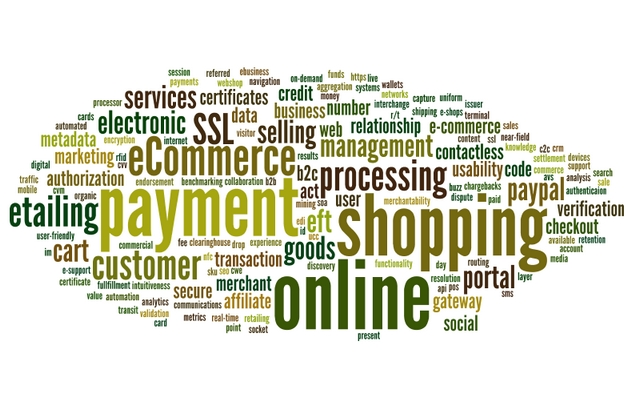
\includegraphics[width=1.0\linewidth]{images/introduction/ecommerce-wordle.jpg}\hfill
 \caption[e-commerce wordle]{e-commerce wordle}
 \label{fig:e_commerce_wordle}
\end{figure}
The increased availability of Internet access and the wide spread of mobile devices has allowed us to consolidate the habit of buying online by customers online already active, that have increased the share of online spending on total consumption.
But what is the correct definition of e-commerce?
\newline
“Commerce is the activity of buying and selling of goods and services, especially on a large scale. The system includes legal, economic, political, social, cultural and technological systems that are in operation in any country or internationally. Thus, commerce is a system or an environment that affects the business prospects of economies. It can also be defined as a component of business which includes all activities, functions and institutions involved in transferring goods from producers to consumers \cite{commerce_def_1}.”
\newline
Other definition:
“Interaction between communication systems, data management systems and security, which because of them exchange commercial information in relation to the sale products or services, will be available, so the definition, the main components of electronic commerce are: communication systems, data management systems and security \cite{commerce_def_2}.”
\newline
In the 1970s, the term electronic commerce, referred to electronic data exchange for sending business documents such as purchase orders and voices electronically. Later, with the development of this industry the term of electronic commerce is used to business of goods and services via the web. When the first World Wide Web was introduced in 1994 as a comprehensive, many well-known researchers have been predicated this type of business “the web-based business” will became soon an important in the world economy, but it took four years that http based protocols should be widely available to users.
The aim of this thesis either to analyze the main systems of e-commerce platforms and either facilitating their realization.
 \newline
Therefore, this thesis is divided in two parts and organized as follows:
Part one consists of five chapters. Chapter One describes the state of the art system of e-commerce and the platforms that their facilitate the realization. Chapter two, analyzes the main companies of e-commerce and the platforms that build systems. Chapter tree analyzes each technology used and describes the methodological approach of each. Fourth chapter analyzes the payment services used. Chapter five provides an overview of Single Page Application development pattern and explains pros and cons and technical functioning.
The second part consists of three chapters. Chapter five describes the project as a whole showing the structure and organization pages. Chapters six is focus on specific components that have been developed, Payment Management and on all the theorical and practical concepts that are behind the ideation of the component. Finally, Chapter seven, exposes project conclusions and further implementations of the work.